\chapter{An�lise do Sistema}

\section{Arquitetura do Sistema}

% Apresentar um diagrama ilustrando:
% - a arquitetura de hardware utilizada, informando para cada hardware o papel dentro da solu��o proposta; 
% - a arquitetura de software utilizada, informando as camadas/m�dulos que ser�o implementados e qual o papel dentro da solu��o proposta.

\subsection{Infraestrutura}

\begin{figure}[ht!]
	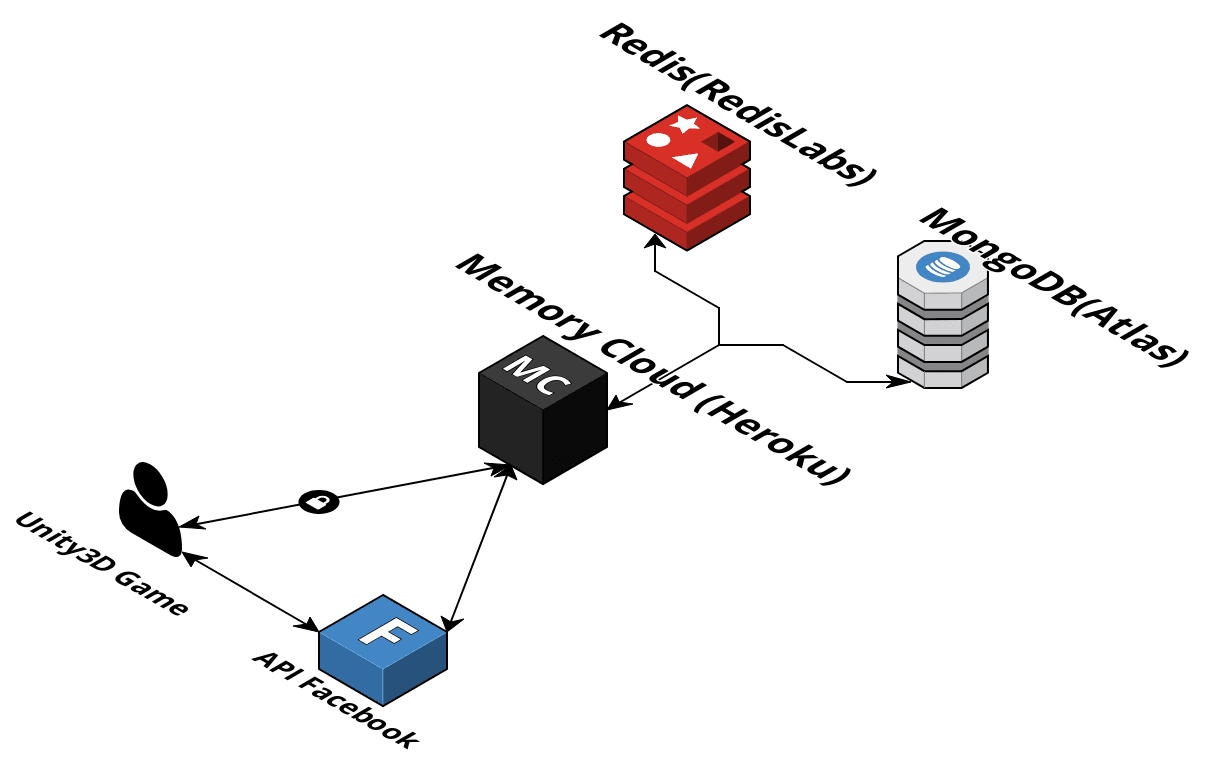
\includegraphics[width=\textwidth]{./5/arquitetura.png}
	\fonte{https://cloudcraft.co}
\end{figure}

\pagebreak

\section{Modelo do Banco de Dados}

\subsection{Modelo Conceitual}

% Apresentar o Diagrama Entidade-Relacionamento desenvolvido para o banco de dados do sistema.

O sistema gerenciador de banco de dados usado � n�o relacional, os dados s�o guardados como documentos em formato JSON.

\subsection{Modelo L�gico}

% Apresentar o esquema relacional (gr�fico ou textual) do banco de dados normalizado e apresentando as tabelas com os atributos e restri��es (chaves).

\begin{figure}[ht!]
	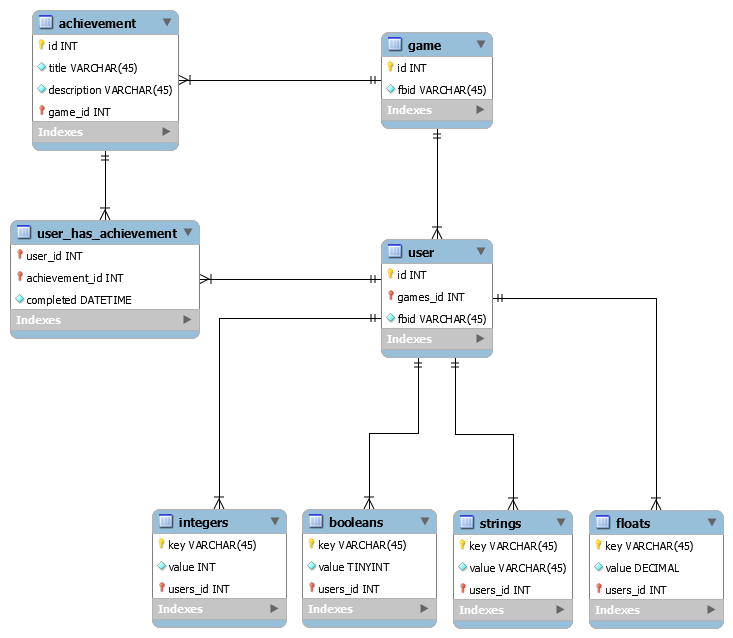
\includegraphics[width=\textwidth]{./5/der.png}
	\fonte{MySQL Workbench}
\end{figure}

\subsection{Dicion�rio de Dados}

% Apresentar o dicion�rio de dados do banco de dados. Documentar cada tabela com seus atributos mostrando nome do atributo, tipo, tamanho, descri��o, se � obrigat�rio ou n�o, e o que mais for necess�rio para descrever os dados. Documentar tamb�m usu�rios, stored procedures, fun��es e qualquer outra implementa��o ligada ao banco de dados.

\begin{figure}[ht!]
	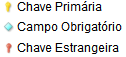
\includegraphics{./5/legenda.png}
\end{figure}

\pagebreak

\section{Diagrama de Classes}

% Apresentar o diagrama de classes completo.

\begin{figure}[ht!]
	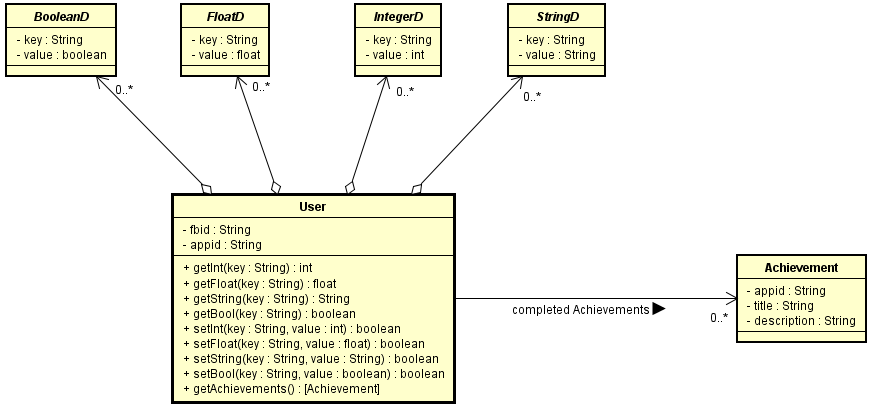
\includegraphics[width=\textwidth]{./5/diagramadeclasses.png}
\end{figure}

\section{Diagrama de Atividades}

% Apresentar o diagrama de atividades, que representa o detalhamento de tarefas e o fluxo de uma atividade para outra de um sistema. Nem todas as tarefas do sistema necessitam de um detalhamento, portanto deve-se considerar no que o diagrama ir� auxiliar na implementa��o do sistema  para decidir quais atividades devem ser descritas.